\documentclass[twoside,11pt]{article}

\usepackage{blindtext}

% Paquetes necesarios
\usepackage{graphicx}
\usepackage{jmlr2e}

% Definiciones útiles
\newcommand{\dataset}{{\cal D}}
\newcommand{\fracpartial}[2]{\frac{\partial #1}{\partial  #2}}

% Encabezados
\usepackage{lastpage}
\jmlrheading{23}{2025}{1-\pageref{LastPage}}{4/25; Revised 5/25}{6/25}{21-0000}{}

\ShortHeadings{Análisis de Mercado Gastronómico en NY}{}
\firstpageno{1}

\begin{document}

\title{Análisis de Mercado Gastronómico en Nueva York para Minimizar el Riesgo de Inversión}

\author{
\name Francisco Lenzik \email francisco@gmail.com \\
\addr Data Scientist
\AND
\name Jerónimo \email jeronimo@gmail.com \\
\addr Data Analyst
\AND
\name Jhon \email jhon@gmail.com \\
\addr Data Analyst
\AND
\name Jorge \email jorge@gmail.com \\
\addr Data Engineer
\AND
\name Jose Quispe \email qjose727@gmail.com \\
\addr Data Engineer
}
\editor{}

\maketitle

\begin{abstract}%   <- trailing '%' for backward compatibility of .sty file
Este reporte presenta el análisis de mercado realizado en Nueva York para el sector gastronómico, con el objetivo de evaluar zonas de la ciudad que minimicen el riesgo de inversión. Utilizando un modelo de Machine Learning y un dashboard interactivo, identificamos los factores clave que impactan en el éxito de las inversiones gastronómicas. El análisis incluye la evaluación de variables socioeconómicas, demográficas y de comportamiento del consumidor en diversas zonas geográficas.
\end{abstract}

\begin{keywords}
  análisis de mercado, riesgo de inversión, Machine Learning, zonas gastronómicas, Nueva York
\end{keywords}

\section{Introducción}

En el sector gastronómico, la toma de decisiones sobre nuevas aperturas de restaurantes y negocios de comida está influenciada por múltiples factores. La evaluación del riesgo de inversión en diferentes zonas geográficas es crucial para minimizar pérdidas y maximizar el retorno. En este reporte, utilizamos un modelo de Machine Learning para analizar diversas variables que afectan el éxito de los negocios gastronómicos en Nueva York.

El objetivo de este proyecto es construir un producto de Machine Learning que identifique las mejores zonas para invertir, reduciendo así el riesgo de fracaso. Para ello, hemos desarrollado un dashboard de análisis interactivo que permite a los usuarios visualizar y explorar diferentes escenarios de inversión en tiempo real.

En este documento, se describen los métodos utilizados para construir el modelo, los datos utilizados en el análisis, y los resultados obtenidos. También se presentan las visualizaciones generadas en el dashboard, las cuales proporcionan información valiosa para los inversores interesados en el sector gastronómico.

\section{Metodología}

Para llevar a cabo este análisis, utilizamos un enfoque de Machine Learning supervisado. Los datos recolectados incluyen información demográfica, socioeconómica y de comportamiento del consumidor en diferentes zonas de Nueva York. Estos datos fueron procesados y utilizados para entrenar un modelo que pueda predecir el éxito de un nuevo negocio gastronómico en función de las características de la zona.

El modelo fue evaluado utilizando técnicas de validación cruzada, y se optimizó utilizando algoritmos como Random Forest y XGBoost. Las variables seleccionadas incluyen la densidad de población, el ingreso promedio por hogar, el nivel de competencia, entre otras.

\section{Resultados}

Los resultados obtenidos a partir del modelo muestran que las zonas con alta densidad de población, mayor poder adquisitivo y menor competencia son las más favorables para nuevas inversiones en el sector gastronómico. A continuación, se presentan las variables más importantes que impactan en el éxito de las inversiones.

\begin{figure}[h] 
    \centering
    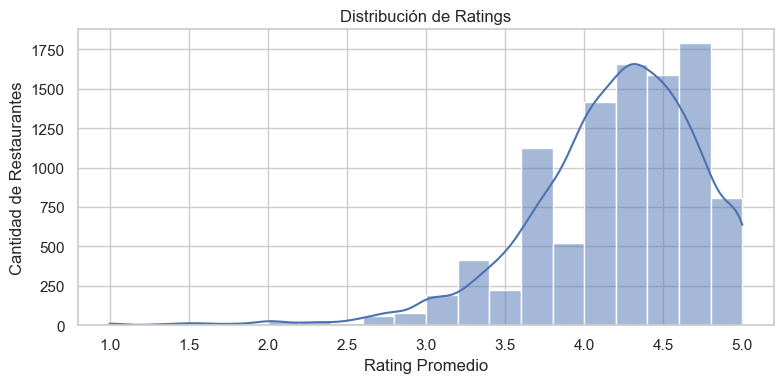
\includegraphics[width=1\textwidth]{importancia_variables.png} 
    \caption{Importancia de las variables en el modelo de Machine Learning}
    \label{fig:importancia_variables} 
\end{figure}

El gráfico anterior muestra la importancia relativa de las diferentes variables utilizadas en el modelo para predecir el éxito de un negocio gastronómico en diversas zonas de Nueva York. Las variables como el ingreso medio por hogar y la densidad de población son las más influyentes, mientras que otras variables como la proximidad a zonas turísticas tienen un impacto moderado.

\section{Dashboard Interactivo}

Para facilitar la toma de decisiones de los inversores, hemos desarrollado un dashboard interactivo que permite visualizar las zonas de Nueva York según las características del análisis. Este dashboard permite a los usuarios explorar diferentes escenarios de inversión y visualizar el riesgo asociado a cada zona. El dashboard también incluye herramientas de filtrado y segmentación de los datos, lo que permite personalizar los análisis según las preferencias del usuario.

\begin{figure}[h] 
  \centering
  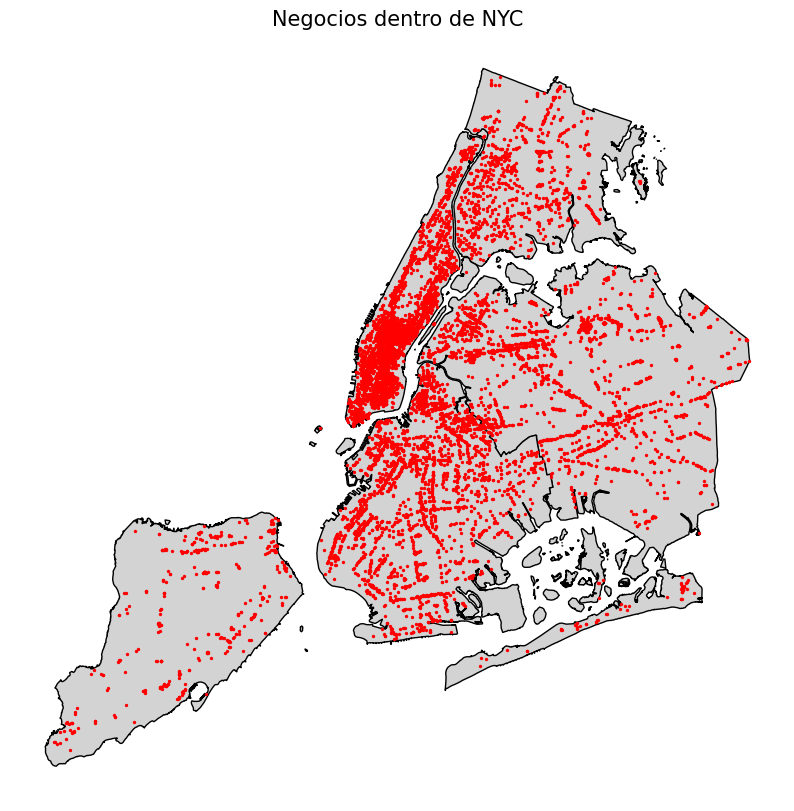
\includegraphics[width=0.6\textwidth]{restaurantes_nyc.png} 
  \caption{Importancia de las variables en el modelo de Machine Learning}
  \label{fig:reataurantes_nyc} 
\end{figure}

\section{Conclusión}

El análisis de mercado realizado en este proyecto ha proporcionado valiosas perspectivas sobre las zonas de Nueva York que ofrecen las mejores oportunidades para nuevas inversiones gastronómicas. El uso de Machine Learning ha permitido identificar de manera precisa las variables más importantes que influyen en el éxito de estos negocios.

Además, el dashboard interactivo desarrollado facilita la toma de decisiones, permitiendo a los inversores analizar en tiempo real las mejores zonas para abrir nuevos restaurantes y negocios gastronómicos. Este proyecto demuestra cómo el análisis de datos y las herramientas de Machine Learning pueden ser utilizadas para minimizar el riesgo de inversión y maximizar el retorno en el sector gastronómico.

\acks{Agradecemos a todos los colaboradores de este proyecto.}

\newpage

\appendix
\section{Modelo de Machine Learning}
\label{app:modelo_ml}

En esta sección se describe en detalle el modelo de Machine Learning utilizado en el análisis, incluyendo la selección de características, los algoritmos empleados y los resultados de la validación cruzada.

\vskip 0.2in
\bibliography{sample}

\end{document}
